\begin{problem}{须弥的山头}{standard input}{standard output}{4.5 seconds}{256 megabytes}

须弥沙漠有许多山,这些山大都无法攀爬,让旅行者感觉很不方便。

众所周知,蒙德城的温迪曾经削掉了蒙德的山头丢进海里以平整地块,并形成了金苹果群岛。

然而温迪不能削掉这些山头,但是他可以帮助你完成\textbf{至多一次}上山。

这些山头都可以被近似认为是多边形,如下图所示,最短路的顶点一定在障碍物多边形的顶点上。

\begin{center}
  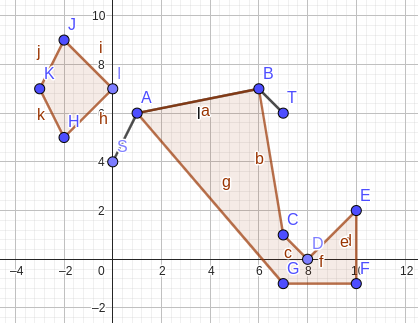
\includegraphics[scale=0.8]{example.png} \\
  \small{一条从$S$到$T$的最短路}
\end{center}

温迪觉得这道题对你来说太难了,所以他帮你处理了几何关系,确切地说,他将告诉你起点,终点,各个多边形的顶点之间是所有无需上山可达的点对,恰好一次上山可达的点对,以及这些点对之间的距离。

看不懂没关系,形式化地,给出一个有红蓝两种边的无向带权图,求至多经过一条蓝边的从起点到终点的最短路。或者断言无论如何都无法到达终点。

\begin{center}
  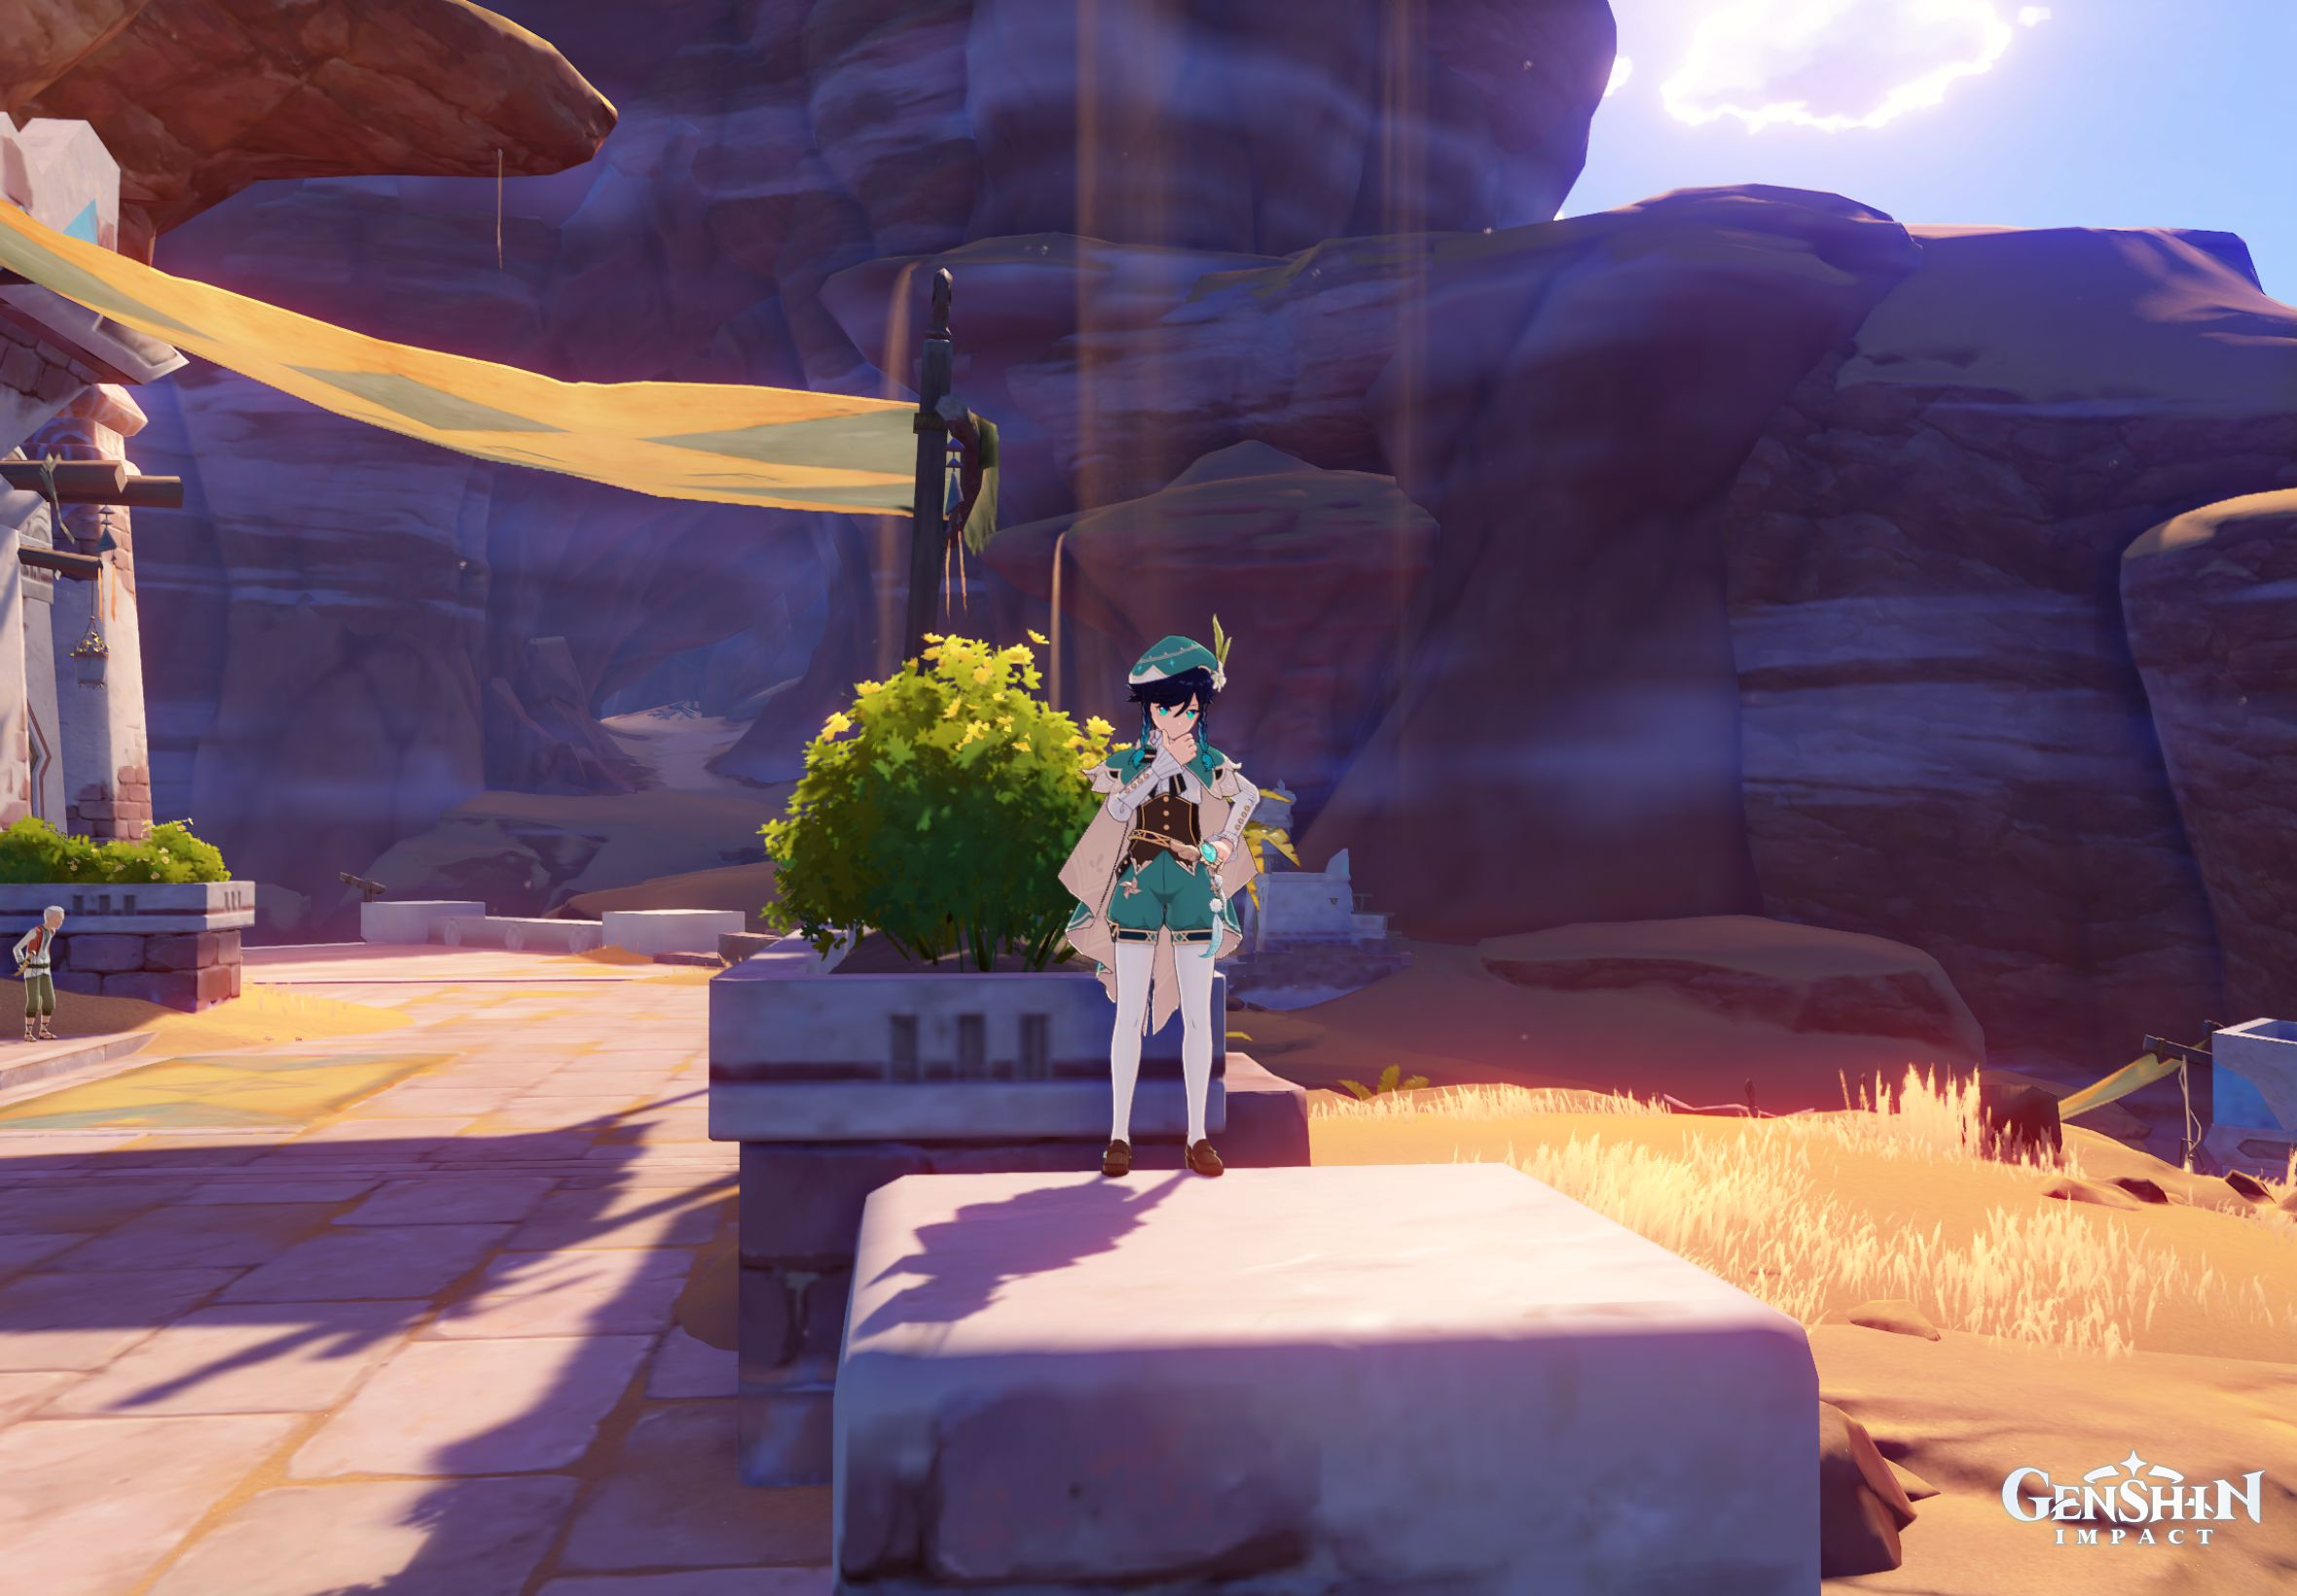
\includegraphics[scale=0.15]{venti.jpg} \\
  \small{温迪可爱!}
\end{center}


\InputFile
第一行三个正整数$n$、$m$、$k$($3 \le n \le 2 \cdot 10^5$,$2 \le m + k \le \min\{\dfrac{(n + 1)(n + 2)}{2}, 2 \cdot 10^5\}$),表示多边形顶点的个数(\textbf {不含起点和终点,编号$3, 4, ..., n + 2$}),无需上山可达的点对的数量(红边数量),恰好一次上山可达的点对的数量(蓝边数量)。

接下来$m$行,每行三个整数$i$、$j$、$w$($1 \le i < j \le n + 2$,$0 \le w \le 10^4$),表示点$i$和点$j$之间无需上山可达(红边),距离为$w$。

接下来$k$行,每行三个整数$i$、$j$、$w$($1 \le i < j \le n + 2$,$0 \le w \le 10^4$),表示点$i$和点$j$之间恰好一次上山可达(蓝边),距离为$w$。


\OutputFile
一个整数,表示起点$1$到终点$2$的最短距离,或者$-1$表示无法到达。

\Examples

\begin{example}
\exmpfile{example.01}{example.01.a}%
\exmpfile{example.02}{example.02.a}%
\exmpfile{example.03}{example.03.a}%
\end{example}

\end{problem}

